\section{Evidence Our Universe is Magnetised}
\label{sec:magnetised-universe}

\subsection{How we reveal the invisible}
\label{sec:how-we-see}

While magnetic fields do not emit radiation directly, their presence can be inferred from the imprint they leave on radiation that has been emitted by and propagated through ionised environments. This inference rests on physics established through laboratory experiments and near-Earth space measurements, which have revealed how magnetic fields influence charged particles and how they modify the polarisation and spectral properties of the radiation we observe. In astrophysics, these same signatures are used to probe and constrain properties of magnetic fields in distant systems, where entire observational surveys are often built around employing a single technique. The catch, however, is that each probe is only sensitive to a particular component of the field, and moreover, the inferred signal is often also impacted by other properties of the medium. Therefore no single observational technique is able to provide a complete view of the cosmic magnetism that threads our Universe. Instead, a coherent picture only emerges once we combine complementary measurements, with the degeneracies of one tracer constrained by another.

Below we discuss a number of observational techniques, highlighting the conditions under which they are useful and which components of magnetic fields they reveal (summarised in \autoref{table:seeing:reqs} and \ref{table:seeing:b-parts}). We then highlight some of the galactic magnetic-fields inferred using these probes in \S\ref{sec:what-we-see}.

\begin{table}
\centering
\caption{Summary of the conditions required for the observational probes discussed below, to produce signatures of cosmic magnetic fields.}
\label{table:seeing:reqs}
\renewcommand{\arraystretch}{1.65}
\begin{tabular}{>{\raggedright\arraybackslash}p{0.3\textwidth} p{0.65\textwidth}}
    \hline
    Probe & Environmental requirements (and limitations) \\
    \hline
    Zeeman splitting (\S\ref{sec:how-we-see:zeeman})
    & Atomic or molecular transitions with narrow, bright spectral lines \\

    Synchrotron radiation (\S\ref{sec:how-we-see:synchrotron})
    & Relativistic electron population; sensitive to beam averaging \\

    Faraday rotation (\S\ref{sec:how-we-see:faraday-rotation})
    & Ionised medium with free electrons along the line of sight; polluted by foreground contamination \\

    Dust polarisation (\S\ref{sec:how-we-see:polarisation})
    & Dust grains in an anisotropic radiation field; affected by line-of-sight and beam averaging \\
    \hline
\end{tabular}
\end{table}

\begin{table}
\centering
\caption{Summary of observational probes and the magnetic field components that they constrain.}
\label{table:seeing:b-parts}
\renewcommand{\arraystretch}{1.65}
\begin{tabular}{>{\raggedright\arraybackslash}p{0.325\textwidth} p{0.625\textwidth}}
    \hline
    Magnetic field component & Observational sensitivity \\
    \hline
    Total field strength, $b$
    & Synchrotron intensity (\S\ref{sec:how-we-see:synchrotron}; indirect; depends on particle population and assumptions, \eg equipartition) \\

    Plane-of-sky field, $b_\perp$
    & Synchrotron polarisation (\S\ref{sec:how-we-see:synchrotron}); dust polarisation (\S\ref{sec:how-we-see:polarisation}; orientation; strength inferred via the Davis-Chandrasekhar-Fermi method) \\

    ``Ordered'' vs ``turbulent'' field structure
    & Synchrotron (de)polarisation (\S\ref{sec:how-we-see:synchrotron}); beam and line-of-sight averaging (\S\ref{sec:how-we-see:polarisation}) \\

    Line-of-sight field, $b_\parallel$
    & Faraday rotation (\S\ref{sec:how-we-see:faraday-rotation}; weighted by thermal electrons); Zeeman splitting (\S\ref{sec:how-we-see:zeeman}) \\

    Large-scale field  coherence
    & Variation of Faraday rotation across sightlines (\S\ref{sec:how-we-see:faraday-rotation}); similarly for polarisation (\S\ref{sec:how-we-see:synchrotron}, and \S\ref{sec:how-we-see:polarisation}) \\

    Small-scale field fluctuations
    & Depolarisation, beam averaging, and frequency-dependent Faraday effects (\S\ref{sec:how-we-see:faraday-rotation}); beam and line-of-sight averaging (\S\ref{sec:how-we-see:synchrotron}, \S\ref{sec:how-we-see:polarisation}) \\
    \hline
\end{tabular}
\end{table}


\subsubsection{Zeeman Splitting}
\label{sec:how-we-see:zeeman}

Zeeman splitting provides one of the most direct ways to measure astrophysical magnetic fields \citep{crutcher2012magnetic, crutcher2019review}. It relies on detecting the Zeeman effect in spectral lines, which is caused by an external magnetic field shifting the energy levels of ions, atoms, or molecules, which leaves a corresponding imprint on the observed spectrum. When detected, this directly constrains the line-of-sight component of the field, $b_\parallel$, which, in contrast to the other probes we discuss below, does not hinge on any assumptions about cosmic-ray populations or energy equipartition, and instead depends directly on the local magnetic field (where the emission took place) \citep{crutcher2012magnetic}; the observed signal is illustrated in \autoref{fig:zeeman}.

\begin{figure}
    \centering
    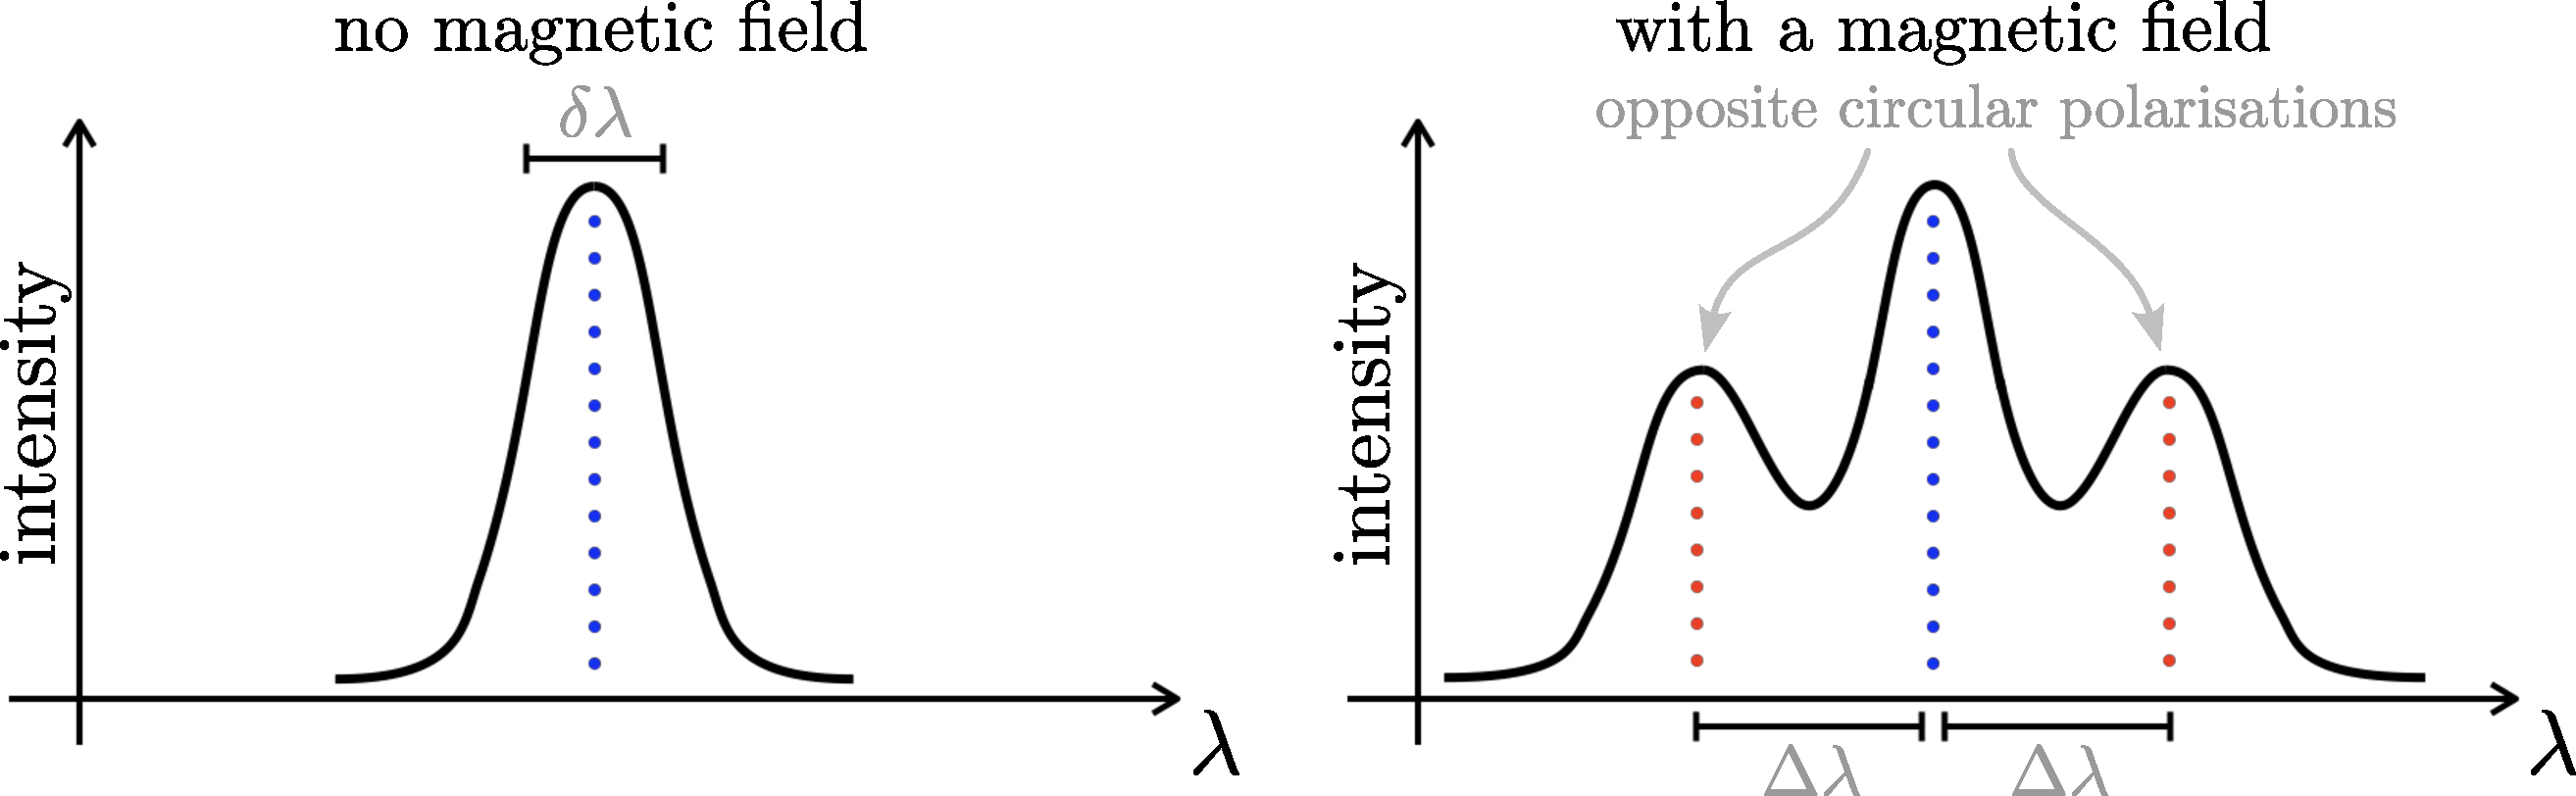
\includegraphics[width=\linewidth]{figures/introduction/zeeman.pdf}
    \caption{Schematic of Zeeman splitting in a spectral line. Without a magnetic field (left), a transition produces a single line with characteristic width $\delta\lambda$ set by thermal and turbulent Doppler broadening. In the presence of a magnetic field (right), the line splits into components with different circular polarisations that are shifted in frequency by $\Delta\lambda \propto b_\parallel$, where $b_\parallel$ is the line-of-sight component of the field. In this figure I have exaggerated the size of the shift for visiblity, but in practice in the interstellar medium, the shift $\Delta\lambda$ is almost always smaller than the intrinsic linewidth $\delta\lambda$, and thus the shift is detected by detecting a residual after differencing the two polarisation components.}
    \label{fig:zeeman}
\end{figure}

This effect arises as a consequence of electrons carrying magnetic moments associated with their spin and orbital motion. In the absence of an external magnetic field, these moments have no preferred orientation, so the magnetic sublevels relevant to a given transition are degenerate, and the transitions only produce spectral lines at a single frequency. However, when an external magnetic field is present, the field couples to the magnetic moments of bound electrons in the emitting or absorbing species, and exerts a torque that causes them to precess about the field's orientation. In these configurations, the field favours orientations that are more closely aligned or anti-aligned, which lifts the degeneracy and shifts the corresponding transition's energy levels by a small amount. In turn, these energy shifts translate into small frequency offsets,
\begin{align}
    \Delta \lambda
        \propto b_\parallel
    ,
\end{align}
in the emitted or absorbed radiation.

Despite its apparent simplicity, Zeeman splitting is not trivial to apply in astronomy \citep[see details by \eg][]{brauer2017magnetic}. This is because the magnitude of the splitting, $\Delta \lambda$, depends on the transition's Zeeman coefficient (set by its effective Land\'e factor), so only a small set of species provide sufficiently large Zeeman sensitivity. In the interstellar medium, where magnetic fields are typically quite weak (at least compared to the plasma environments we can create in laboratories on Earth), this limits us to tracers like the atomic hydrogen 21-cm transition and molecules with large electronic magnetic moments, like OH, CN, CH, CCS, SO, and O$_2$. However, even for these tracers, $\Delta \lambda$ is usually much smaller than the observed line width $\delta \lambda$ set by thermal (and turbulent) Doppler broadening, so the Zeeman components are rarely resolved as separate peaks.

In practice, one therefore measures the associated circular-polarisation signature across the line profile. The split Zeeman components carry opposite circular polarisations, so splitting the signal into left- and right-circular polarisations and differencing them yields a characteristic antisymmetric residual whose amplitude is proportional to $b_\parallel$. Because many instrumental and sky-noise contributions enter both polarisation channels in a similar way, differencing suppresses the shared noise-modes and allows detection of much weaker splitting than would be possible from total intensity alone. Where it can be applied, Zeeman splitting provides a uniquely direct constraint on $b_\parallel$, which can be used to calibrate and validate field estimates inferred from synchrotron emission and Faraday rotation.

\subsubsection{Synchrotron Radiation}
\label{sec:how-we-see:synchrotron}

At radio wavelengths, synchrotron radiation from relativistic electrons provides one of the most widely used tracers of cosmic magnetism \citep{vallee2011magnetic}. As these electrons propagate through magnetised environments, their trajectories are bent by magnetic tugs (the Lorentz force) into gyrating trajectories about magnetic field lines. Since these particles experience a constant acceleration, they radiate, and since they are relativistic, their radiation is strongly beamed along the instantaneous direction of motion. An ensemble of gyrating electrons then produces diffuse radiation whose intensity depends on the magnetic field strength, $b$, and on the energy distribution of the radiating electrons, while its polarisation traces the geometry of the plane-of-sky component, $b_\perp$. \autoref{fig:synchrotron} illustrates the basic geometry of this process.

\begin{figure}
    \centering
    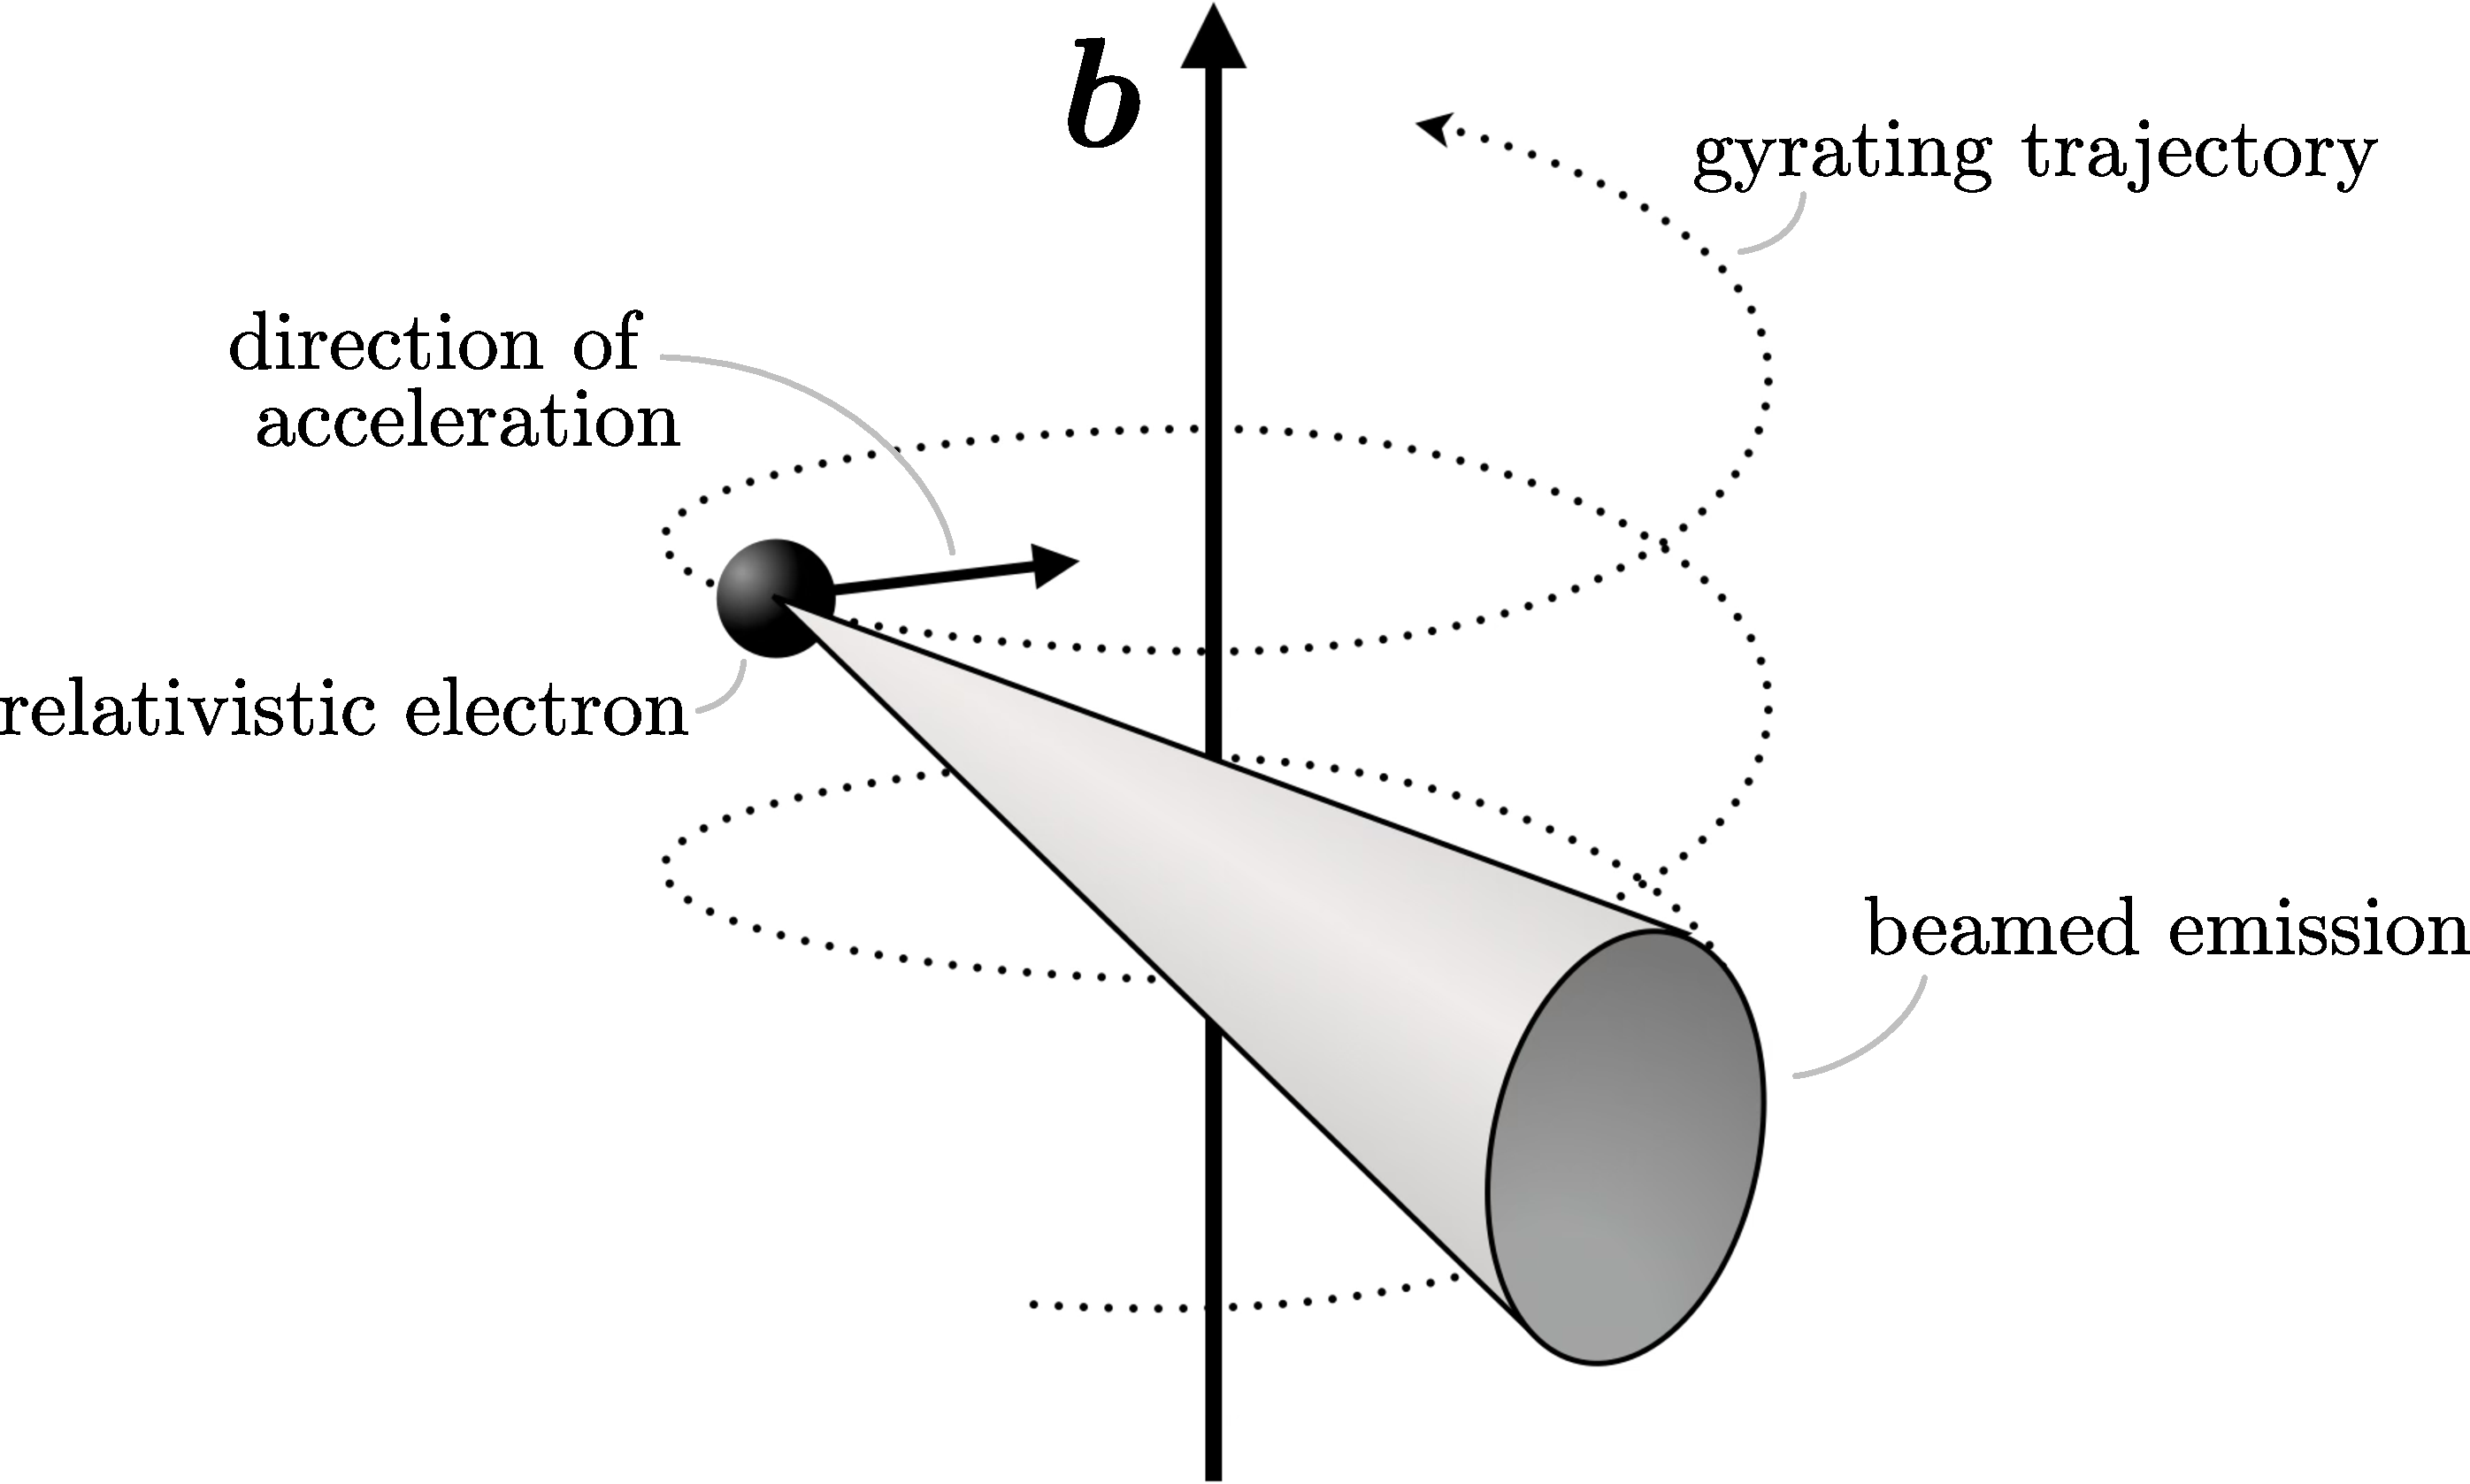
\includegraphics[width=0.85\linewidth]{figures/introduction/synchrotron.pdf}
    \caption{Schematic of synchrotron emission, adapted from \citet{shukurov2021astrophysical}. A relativistic electron gyrates about a magnetic field, $\mVector{b}$, with the Lorentz force providing an acceleration directed toward the local centre of its trajectory. Because the electron is relativistic, the emitted radiation is strongly beamed along the instantaneous direction of motion, producing a narrow emission cone.}
    \label{fig:synchrotron}
\end{figure}

At longer radio wavelengths ($\lambda \sim \mathrm{cm}-\mathrm{m}$), synchrotron emissivity depends on the relativistic electron population and the magnetic field strength,
\begin{align}
    \epsilon_\lambda
        \propto n_\mathrm{re}\, b^{(p+1)/2}\, \lambda^{(p-1)/2}
    ,
\end{align}
for an electron energy distribution $\mdd n / \mdd E_e \propto E_e^{-p}$, where $n_\mathrm{re}$ is the relativistic electron number density, and $p$ is the electron spectral index. Synchrotron emission therefore constrains $b$ only in combination with $n_\mathrm{re}$. The intensity alone cannot be inverted to a magnetic field strength without a closure for $n_\mathrm{re}$ (or, more generally, for the cosmic-ray electron energy density). However, a common closure, and perhaps the simplest choice, is to assume an approximate equipartition between the energy densities of cosmic rays and magnetic fields \citep{beck2005revised}, which yields a practical estimate of $b$, but inherits uncertainty from assumptions about the particle spectrum, filling factors, and the degree to which local energy balance holds true \citep{seta2019revisiting}.

Synchrotron emission is intrinsically linearly polarised, and so polarisation angle provides a second observable probe, alongside the total intensity, revealing the orientation of the ordered component of $b_\perp$. That said, the measured angle is not, in general, the same as the emission angle, because propagation through a magnetised plasma can rotate the plane of polarisation (see Section~\ref{sec:how-we-see:faraday-rotation}). Moreover, the polarisation fraction is also often suppressed, since the observed signal could contain many emitting regions along the line-of-sight (and across the telescope beam), so polarisation contributions may partially cancel. Polarisation, therefore, tends to mainly diagnose the degree of ordering in $b_\perp$, but cannot by itself tell whether the ordered component reflects a truly coherent field, or an anisotropically aligned, turbulent one.

At higher energies, relativistic electrons can also produce X-ray emission through inverse Compton scattering, which in some environments provides a useful complement to synchrotron measurements. For example, in radio-galaxy lobes (where seed photons are dominated by the cosmic microwave background) and in compact hotspots (where synchrotron self-Compton emission can apply), magnetic field strengths can be constrained from the ratio of synchrotron to inverse-Compton flux \citep[see reviews by \eg][]{worrall2002gaseous, hardcastle2020radio}.

\subsubsection{Faraday Rotation}
\label{sec:how-we-see:faraday-rotation}

Faraday rotation probes magnetic fields through their effect on the propagation of linearly polarised radiation, and explains why the polarisation angle (the orientation of the projected electric-field vector) inferred from synchrotron emission may be different from its emitted angle \citep{brentjens2005faraday}. This is because, as polarised radiation propagates through an ionised medium, the linear polarisation plane rotates by an amount proportional to $\lambda^2$, where $\lambda$ is the wavelength of the light (this is illustrated in \autoref{fig:faraday}). The rate of this rotation is quantified by the rotation measure,
\begin{align}
    \mathrm{RM}
        \propto \int n_\mathrm{th}\, b_\parallel \, \mdd l
    , \label{eqn:how-we-see:RM}
\end{align}
where $n_\mathrm{th}$ is the thermal (free) electron number density, and $b_\parallel$ is the line-of-sight component of the magnetic field \citep{haverkorn2014magnetic}. Faraday rotation therefore constrains $b_\parallel$ through the magnitude and sign of $\mathrm{RM}$, but only in combination with an understanding for the thermal electron distribution, since the integral in \autoref{eqn:how-we-see:RM} is weighted by $n_\mathrm{th}$ and by the path length through the plasma.

\begin{figure}
    \centering
    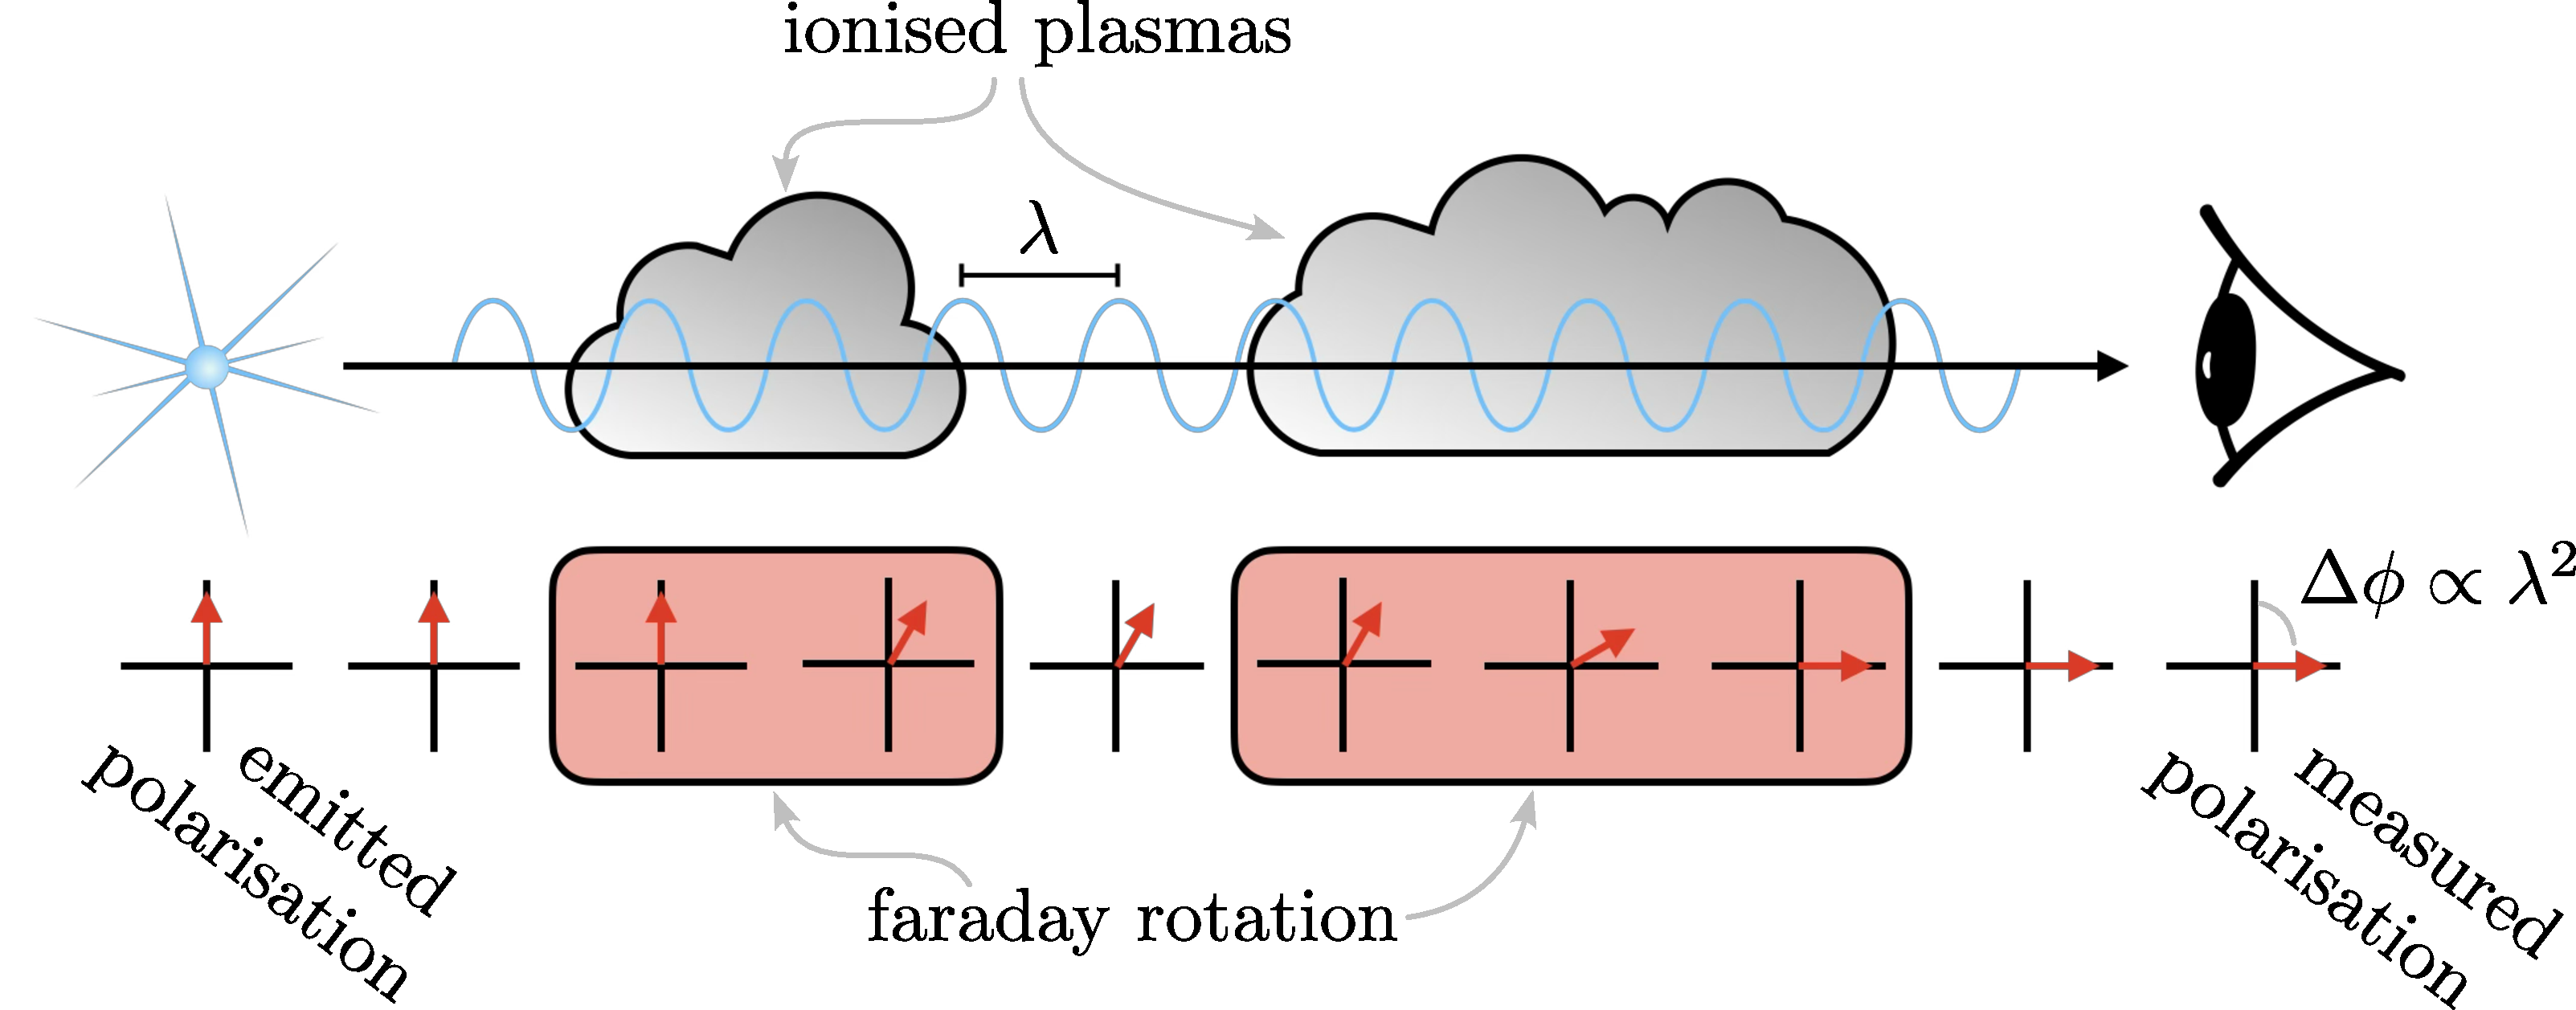
\includegraphics[width=\linewidth]{figures/introduction/faraday.pdf}
    \caption{Schematic of Faraday rotation. Linearly polarised radiation emitted by a background source propagates through regions of ionised plasma, causing the polarisation angle, $\phi$, to rotate. The accumulated rotation depends on wavelength as $\Delta\phi \propto \lambda^{2}$, with the rate of rotation quantified by the rotation measure (see \autoref{eqn:how-we-see:RM}).}
    \label{fig:faraday}
\end{figure}

In realistic astrophysical plasmas, however, $b_\parallel$ can reverse many times along the line of sight, so positive and negative contributions often lead to integrated $\mathrm{RM}$ that nearly cancel \citep{haverkorn2014magnetic}. As a consequence, in practice, $\mathrm{RM}$ primarily traces the net, large-scale component of $b_\parallel$, while small-scale structures are imprinted as fluctuations in $\mathrm{RM}$ across neighbouring sightlines, and as depolarisation of the polarised emission. Interpreting $\mathrm{RM}$ in terms of a field strength therefore benefits from independent constraints on $n_\mathrm{th}$, and from combining Faraday rotation with synchrotron intensity and polarisation to jointly constrain $b_\parallel$ and $b_\perp$.

\subsubsection{Dust Polarisation}
\label{sec:how-we-see:polarisation}

\begin{figure}
    \centering
    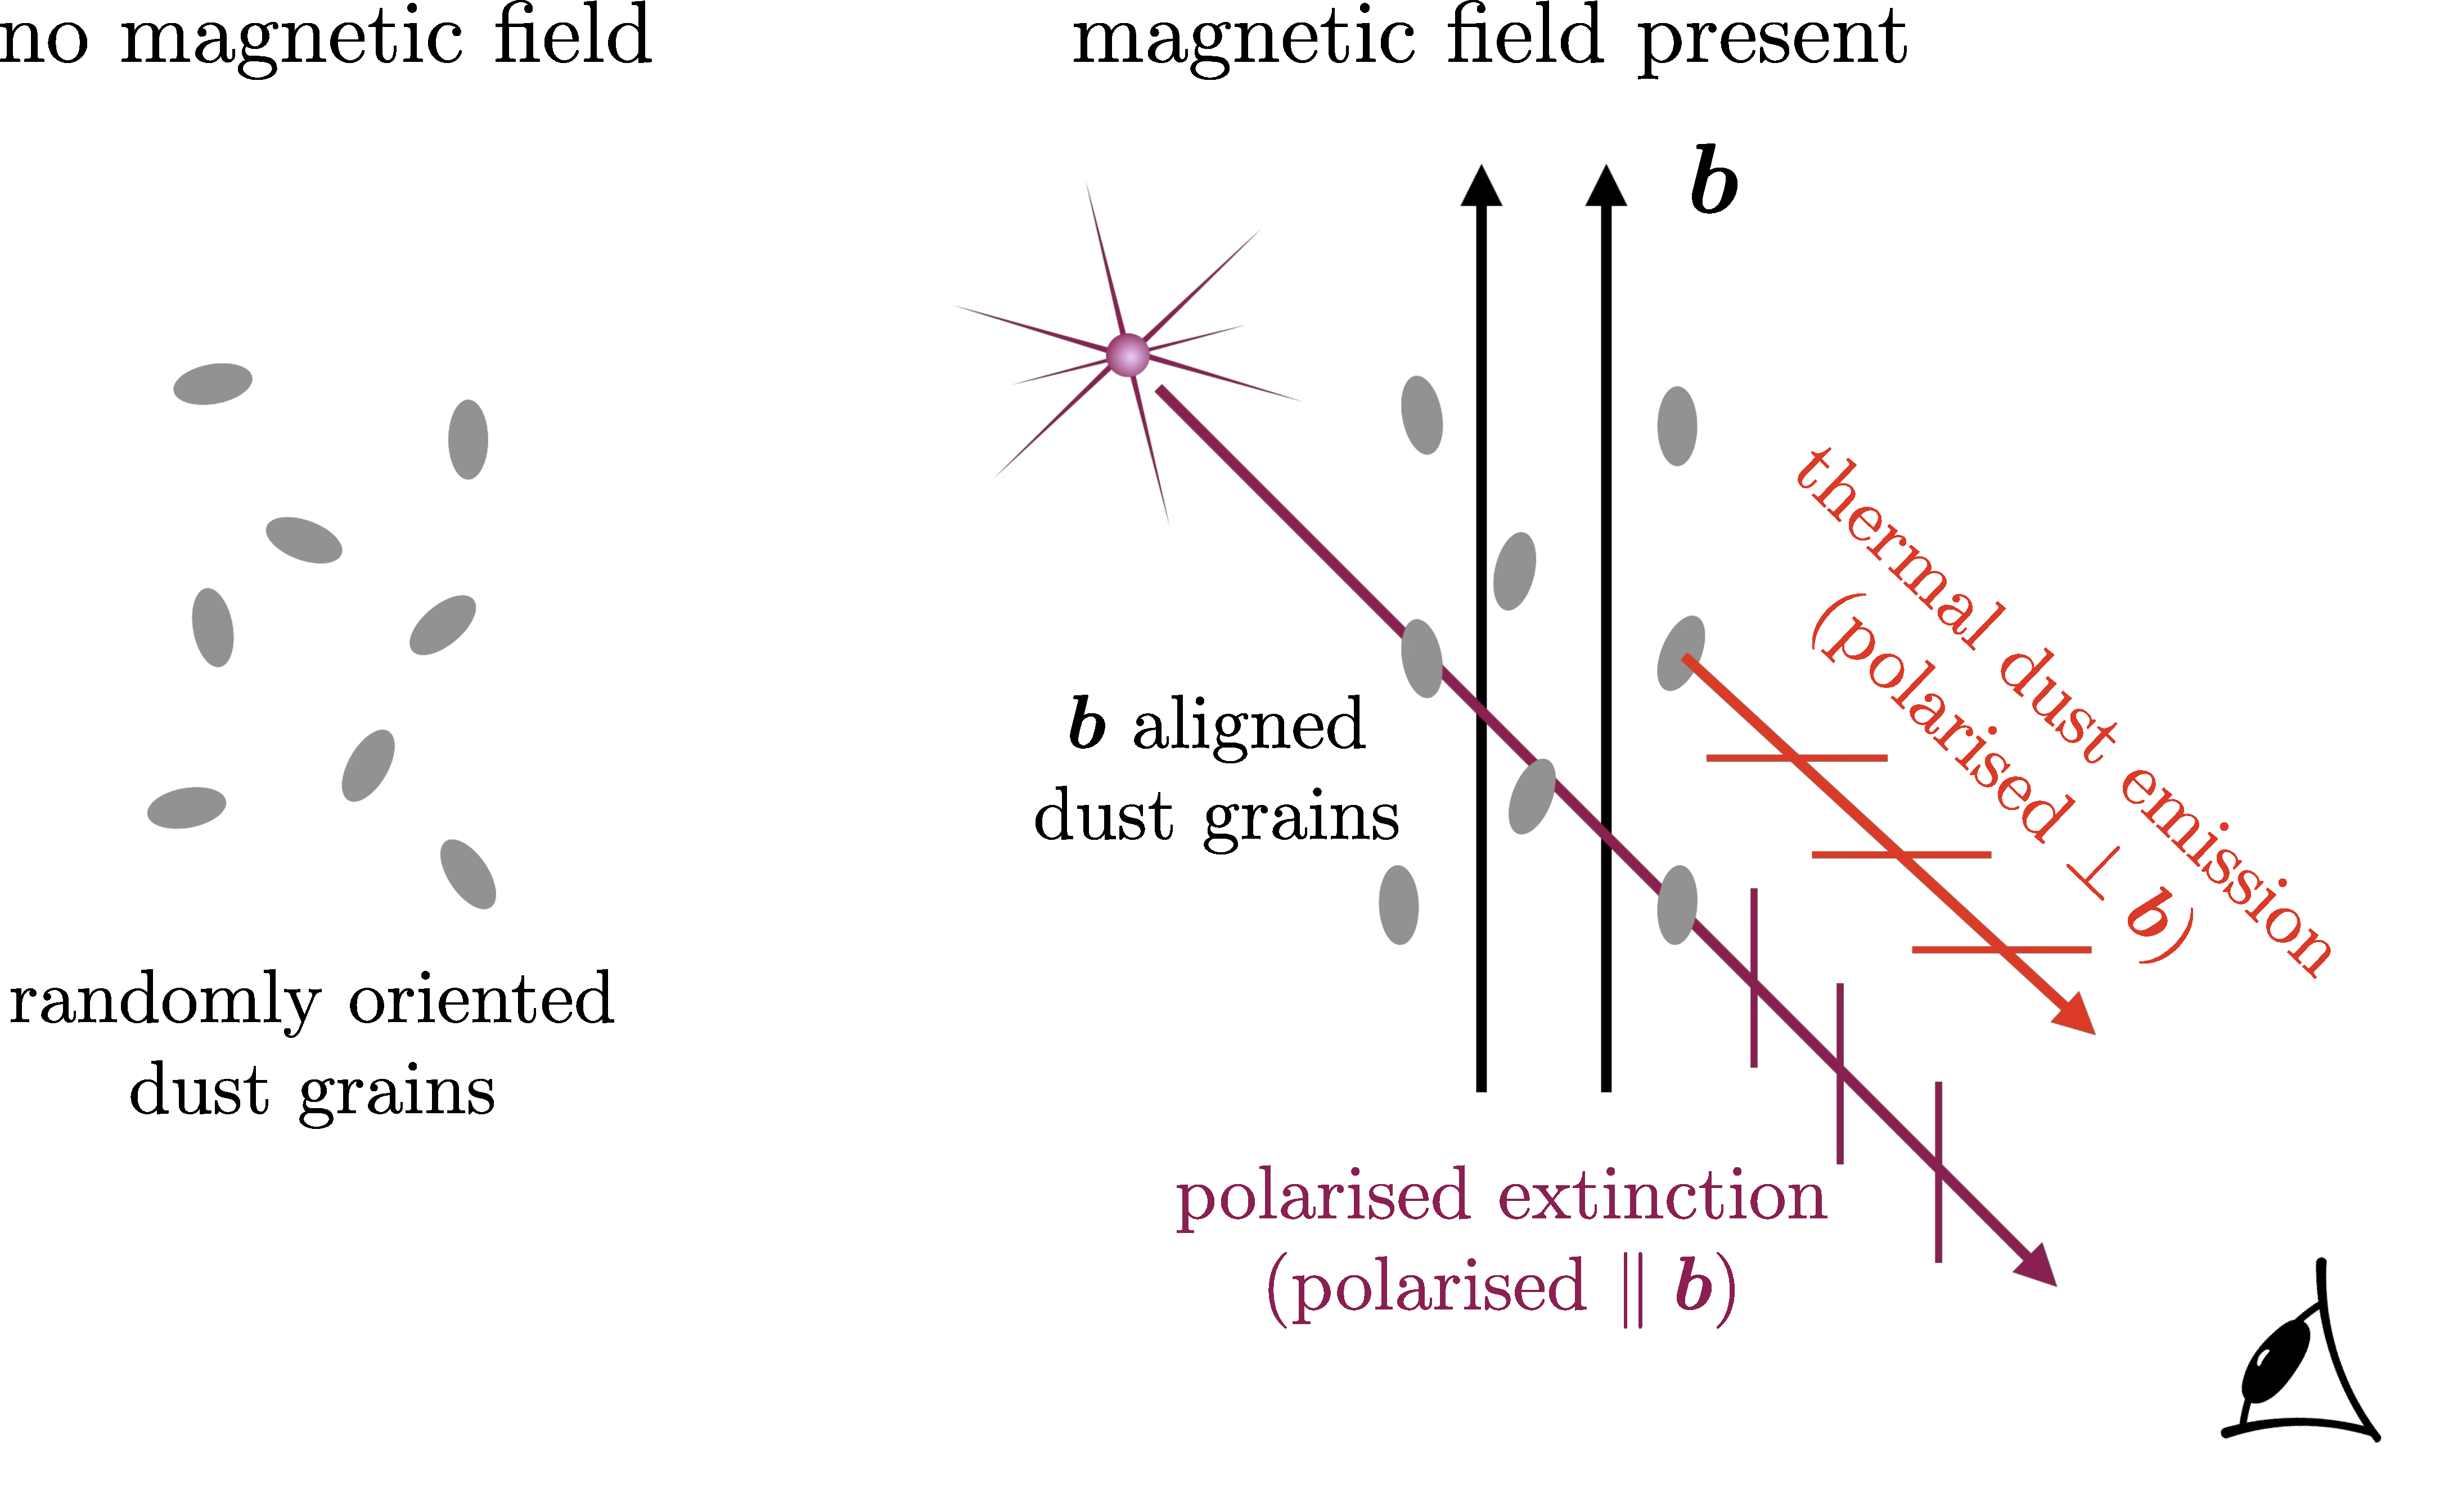
\includegraphics[width=\linewidth]{figures/introduction/dust.pdf}
    \caption{Schematic of dust polarisation, adapted from a lecture by Jennifer Schober. In the absence of a magnetic field (left), dust grains are randomly oriented and produce little net linear polarisation. When a magnetic field is present (right), elongated grains become preferentially aligned with the local field direction, $\mVector{b}$, so that both polarised extinction of background starlight (with polarisation aligned parallel to $\mVector{b}$) and polarised thermal emission (with polarisation aligned perpendicular to $\mVector{b}$) can be used to trace magnetic-field orientation.}
    \label{fig:dust}
\end{figure}

The final probe we will discuss is dust polarisation, which, like synchrotron polarimetry, traces the plane-of-sky magnetic field component, $b_\perp$, through measurements of linear polarisation. At far-infrared and sub-millimeter wavelengths\footnote{
    Faraday rotation is typically negligible at these wavelengths. To see why, consider \autoref{eqn:how-we-see:RM} for a typical diffuse ISM sightline, where $n_\mathrm{th}\sim 0.03~\mathrm{cm^{-3}}$, $b_\parallel\sim 3~\mu\mathrm{G}$, and $L\sim 1~\mathrm{kpc}$. With this, an order-of-magnitude analysis gives $\mathrm{RM}\sim 10^2~\mathrm{rad\,m^{-2}}$. Since the amount of rotation scales as $\lambda^2$, an order-unity rotation requires $\lambda \gtrsim 10^{-1}~\mathrm{m}$, and therefore, at wavelengths associated with dust polarisation, namely $\lambda \lesssim 10^{-3}~\mathrm{m}$, rotation is suppressed; for the same sightline, the rotation at $\lambda\lesssim 10^{-3}~\mathrm{m}$ is smaller than at $\lambda\sim 10^{-1}~\mathrm{m}$ by a factor $\left(10^{-3}/10^{-1}\right)^2 \sim 10^{-4}$, so dust polarisation can usually be interpreted without an $\mathrm{RM}$ correction.
    \label{fnote:faraday}
}, these polarisation measurements are dominated by thermal emission from interstellar dust grains, whereas, at optical and near-infrared wavelengths, they are dominated by the polarised extinction of background starlight by dust. In both regimes, a preferred polarisation emerges because interstellar grains are charged and typically elongated rather than spherically symmetric, which leads to them becoming preferentially aligned with the local magnetic field \citep{andersson2015interstellar}. This alignment makes their absorption and emission anisotropic, producing linearly polarised radiation whose orientation traces the ordered component of $b_\perp$ in the dust-bearing gas (see \autoref{fig:dust}).

Because dust is abundant in the cold and warm phases of the interstellar medium, particularly in filaments and star-forming clouds, dust polarisation is often the most effective cartographer of $b_\perp$ in these environments \citep{collaboration2015planck}. However, dust polarisation on its own only provides a very limited direct constraint on field strength, since the polarisation fraction does not only depend on the field geometry, but also on dust grain properties, alignment efficiency, and line-of-sight averaging. Its primary utility is therefore in constraining the orientation and coherence of $b_\perp$ in dense, dusty environments where synchrotron emission may be weak and Faraday rotation may be hard to interpret.

The \textit{structure} of polarisation maps can nevertheless be used to obtain an estimate of $b_\perp$, where a popular approach is the Davis-Chandrasekhar-Fermi method \citep{davis1951polarization, chandrasekhar1953magnetic}, in which turbulent motions are assumed to perturb the plane-of-sky field, producing a dispersion in polarisation angles, $\sigma_\phi$, whose magnitude reflects the ratio of turbulent to magnetic restoring stresses. Combining $\sigma_\phi$ with an estimate of the gas mass density, $\rho$, and a one-dimensional velocity dispersion, $\sigma_u$, inferred from line widths yields an order-of-magnitude estimate,
\begin{align}
    b_\perp
        \sim Q \, \sqrt{4\pi\rho} \, \frac{\sigma_u}{\sigma_\phi}
    ,
\end{align}
where $Q$ is an order-unity calibration factor that absorbs geometric and line-of-sight effects \citep[\eg][]{ostriker2001density}.

\subsection{A (Brief) Excursion Through Astrophysical Plasmas}
\label{sec:what-we-see}

Zeeman splitting has been successfully applied to star-forming, dense molecular clouds, where measurements indicate $b \sim 10-100 \,\mu\mathrm{G}$ in regions undergoing active collapse and feedback (\eg \citealt{sarma2013very}; see also, \eg \citealt{pattle2022magnetic} for a thorough review). Independent dust polarisation and Faraday-based observations are consistent with these estimates, and indicate that the orientation of $b$ remains ordered over entire clouds, at least on scales of $\sim 10 \,\mathrm{pc}$ \citep{collaboration2015planck, fissel2016balloon, tahani2018helical}. Moreover, dust polarisation measurements at far-infrared wavelengths ($\lambda \sim 50-200 \,\mu\mathrm{m}$) extend this picture to denser regions of the Milky Way, revealing similarly ordered magnetic structures in dense, dust-obscured regions of active star formation \citep{lopez2020sofia}. These different probes and surveys point to a common conclusion for magnetic fields in the Milky Way's dense ISM and star-forming clouds: magnetic energy densities fluctuate about equipartition with kinetic and gravitational energy densities. However, one needs to be careful interpreting these measurements directly, since numerical simulations have shown that projection effects and intermittency can complicate the mapping between observed and intrinsic field properties \citep{camacho2023kinetic, hu2023sub, seta2025magnetic}.

Beyond the Milky Way, nearby spiral galaxies provide some of the clearest evidence for galactic magnetic fields. In the grand-design spiral galaxy M51, for example, synchrotron polarisation and rotation measure observations at $6 \,\mathrm{cm}$ reveal a magnetic field organised on $\sim \mathrm{kpc}$ scales, closely tracing the spiral arms of the disc \citep{fletcher2011magnetic}. In contrast, dust polarisation measurements at $154 \,\mu\mathrm{m}$ reveal a field that varies on $\sim 10 \,\mathrm{pc}$ scales across regions of dense molecular ISM \citep{borlaff2021extragalactic}. These measurements (see \autoref{fig:m51}) probe different phases of the ISM, with dust polarisation tracing cold, dense gas that is sensitive to the plane-of-sky orientation of $b$, while synchrotron emission and Faraday rotation sample diffuse magnetised plasma distributed across the disc. The coexistence of these signatures suggests that the galactic magnetic field carries a large-scale component organised across the disc, alongside a component that varies across the turbulent, star-forming ISM. Similar dust polarisation observations with ALMA show that this is not unique to M51, and is instead a common feature of present-day spiral galaxies \citep[\eg][]{belfiori2025dust, de2025grand}.

\begin{figure}
    \centering
    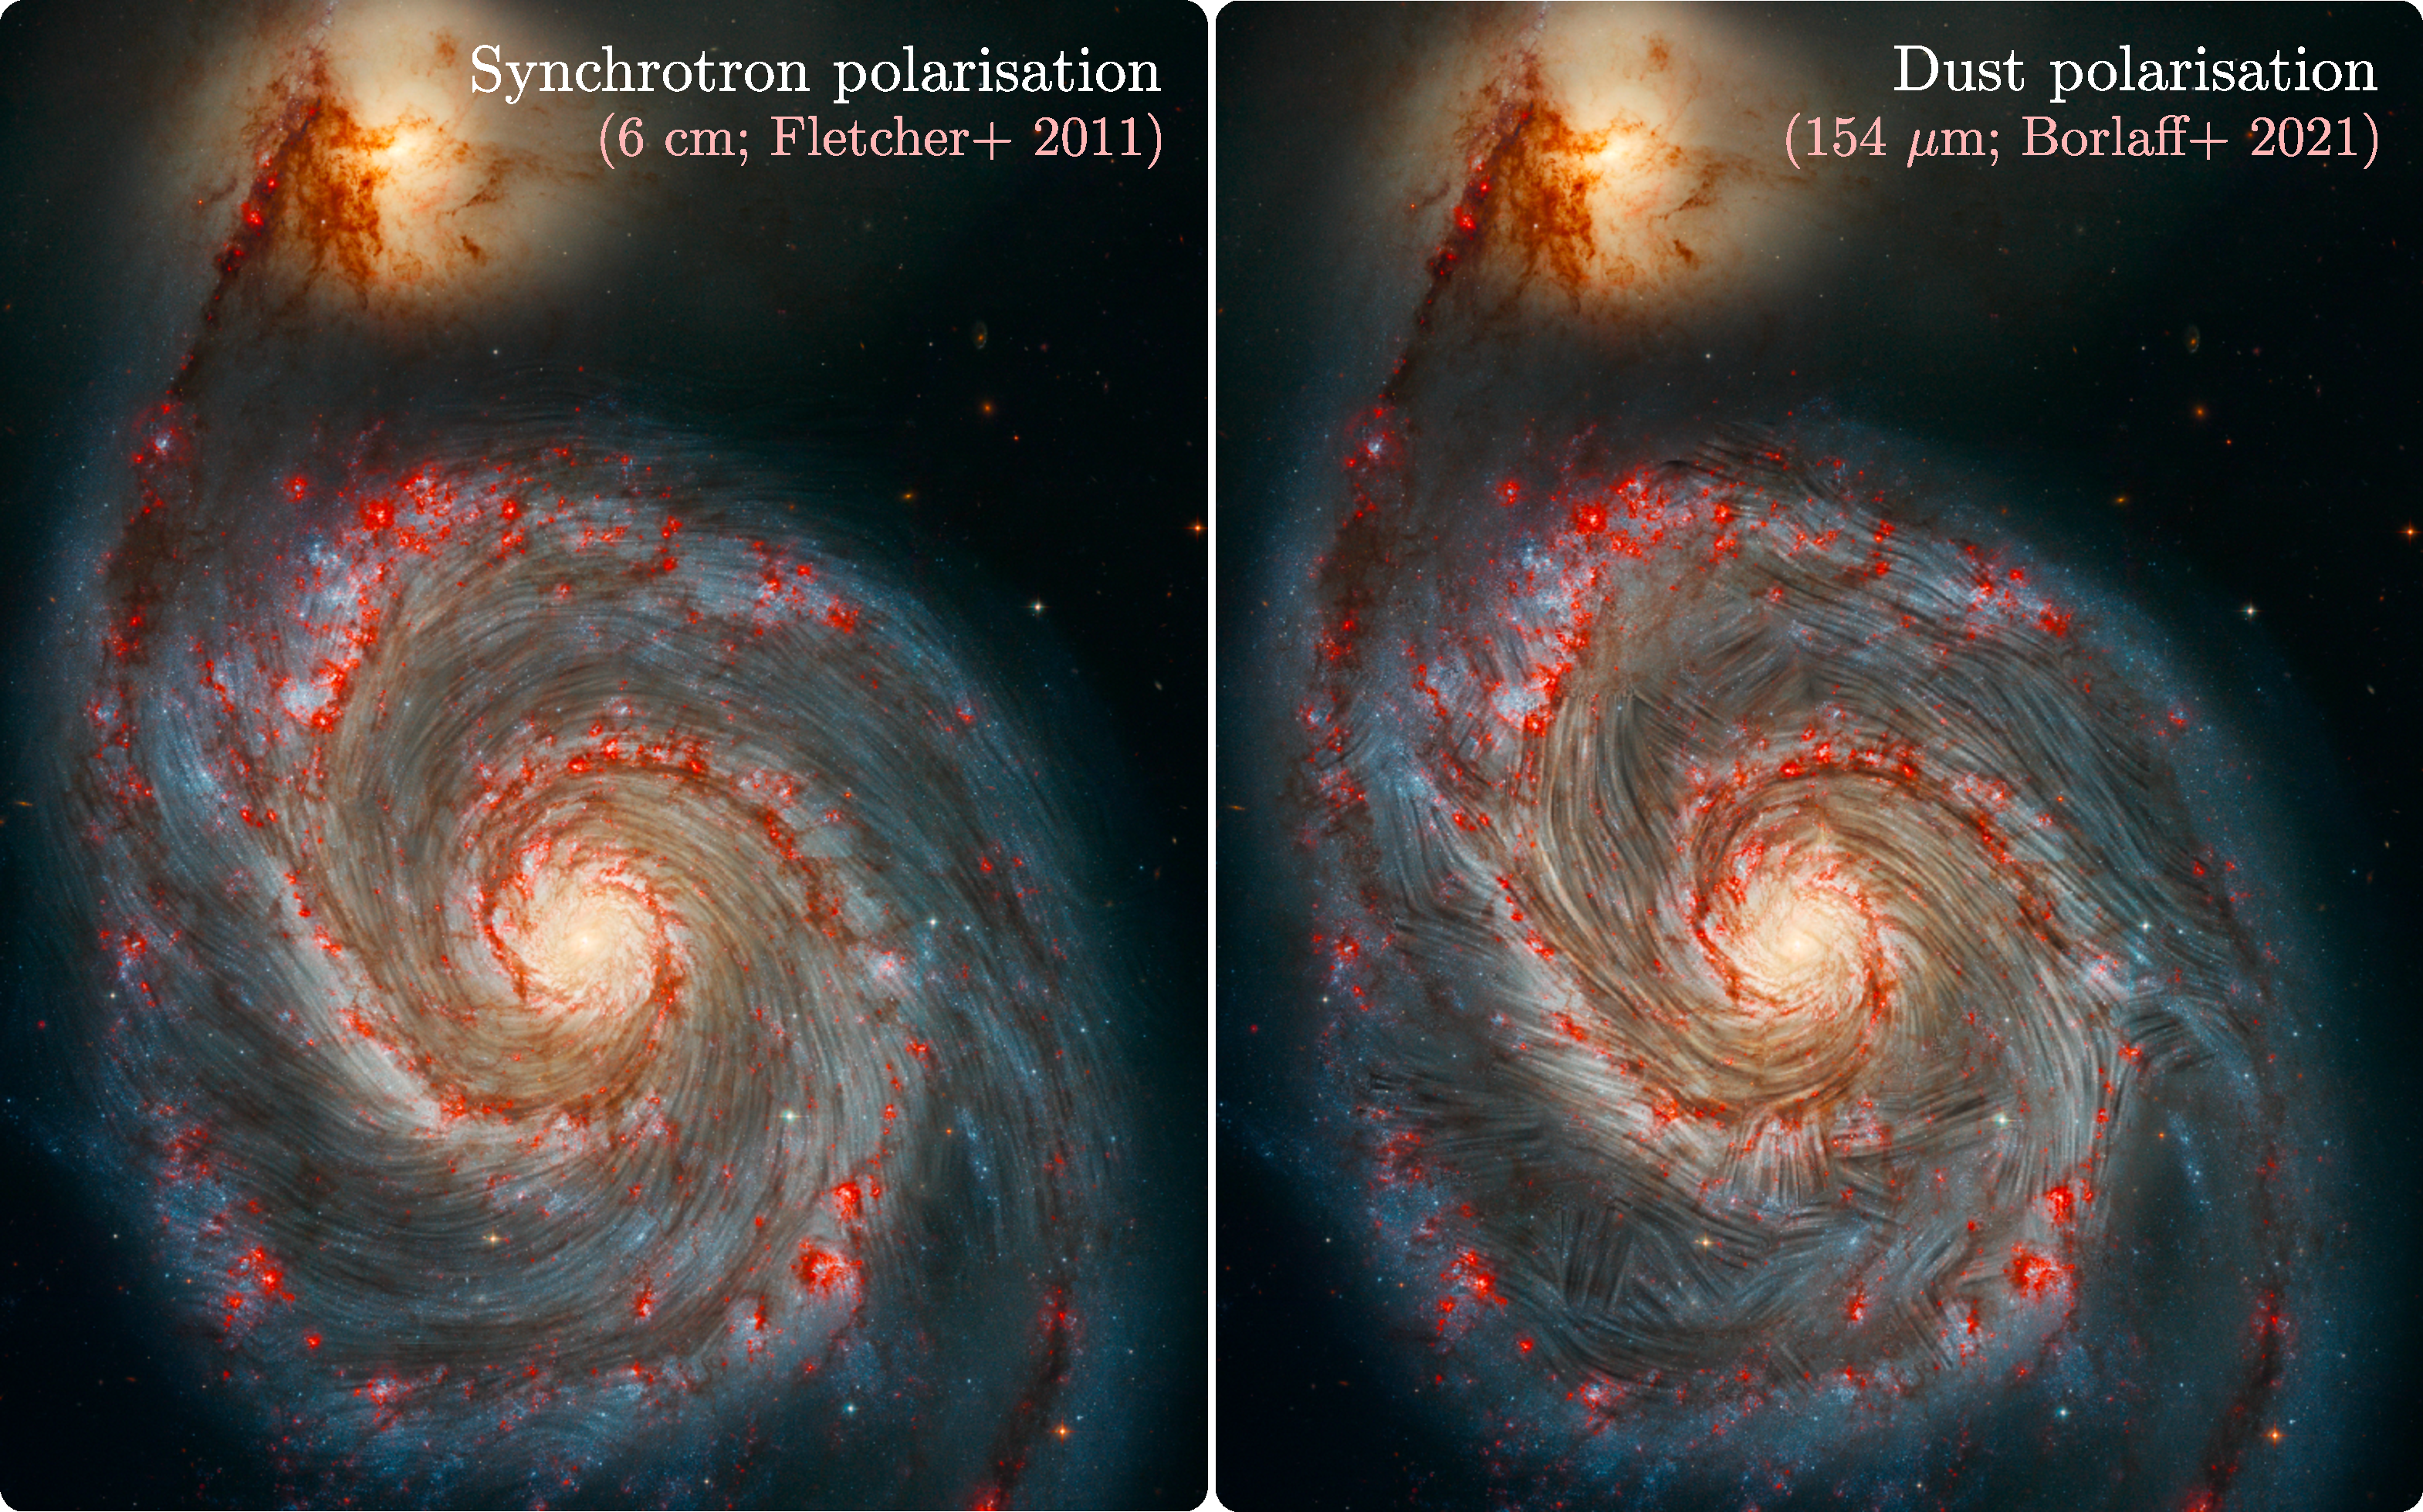
\includegraphics[width=\linewidth]{figures/introduction/M51.pdf}
    \caption{Plane-of-sky magnetic-field orientation in M51 inferred from polarised emission tracing different phases of the interstellar medium. In the left panel, synchrotron polarisation measured at $6\,\mathrm{cm}$ probes the ordered component of the plane-of-sky field, $b_\perp$, in diffuse magnetised plasma \citep{fletcher2011magnetic}; in the right panel, dust polarisation at $154\,\mu\mathrm{m}$ samples colder, denser gas \citep{borlaff2021extragalactic}. In both cases, the polarisation angle constrains the orientation of $b_\perp$ (with only the synchrotron angle susceptible to Faraday rotation along the line of sight; see \autoref{fnote:faraday}).}
    \label{fig:m51}
\end{figure}

Perhaps the most surprising observational result, which, as we discuss below, sits at odds with the current picture of magnetogenesis, is that coherent magnetic fields already appear to be present on $\sim\mathrm{kpc}$ scales in ``young'' galaxies. Rotation-measure studies at $z \sim 1$ indicate ordered line-of-sight field components comparable to those in nearby systems \citep{bernet2008strong, sur2018faraday}. More recently, ALMA detections of polarised dust emission have extended this picture to earlier epochs, revealing ordered plane-of-sky magnetic structures at $z \approx 2.6$ and $z \approx 5.6$ on scales of several $\mathrm{kpc}$ \citep{geach2023polarized, chen2024kiloparsec}. This is particularly surprising, because these ordered fields are usually associated with mechanisms that rely on sustained coherent rotation to organise magnetic structure on galactic scales. These galaxies, however, are placed at epochs where rotationally supported discs are generally not expected to have fully formed (\citealt{geach2023polarized} estimate a dynamo number $\mathcal{D} \approx 3$; see \S\ref{sec:evolve:lsd}). The presence of coherent magnetic fields at such early times therefore poses a significant challenge, and motivates a closer exploration of the circumstances and conditions under which large-scale magnetic structures could be generated in young systems.
